% This file (thesis-main.tex) is the main file for a master's thesis.
\documentclass {udthesis}

% preamble

% Include graphicx package for the example image used
% Use LaTeX->PDF if including graphics such as .jpg, .png or .pdf.
% Use LaTeX->PS->PDF if including graphics such as .ps or .eps
% Best practice to not specify the file extension for included images,
% so when LaTeX is building it will look for the appropriate image type.
\usepackage{graphicx}
\usepackage[margin=1in]{geometry}
\usepackage{float}
\usepackage{wrapfig}
\usepackage{tcolorbox}
\usepackage{booktabs}
\usepackage{tabularx}

\usepackage{graphicx} % Required for inserting images


\usepackage{mdframed}
\usepackage{xcolor}
\usepackage[
    backend=biber,
    style=ieee,
  ]{biblatex}
\addbibresource{sources.bib}
\addbibresource{sample.bib}


\newtcolorbox{commentbox}{
boxrule=0pt,
colback=yellow!40!white,
sharp corners
}
\newtcolorbox{questionbox}{
boxrule=0pt,
colback=blue!40!white,
sharp corners
}
                
\begin{document}
% 
% This is the Title and Approval Page file (thesis-tap.tex) for
% a master's thesis.
%
% The order of the commands below is very important.
% You may choose to add or eliminate a \prefacesection 
% in the front material but the order should remain 
% the same especially \maketocloflot followed by 
% \prefacesectiontoc{Abstract}

% Title and author are also used for PDF file properties
% No special character or commands can be used for the PDF definition; 
% use the [options] paramater to specify a different title or author 
% to remove special characters or commands like \\ for example.
\title[Machine Learning in Imaging: Automated Phenotyping in Plant Science]{Machine Learning in Imaging:\\
Automated Phenotyping in Plant Science}
\author{Joseph Cristiano}
\type{thesis}
\degree{Master of Science}
\majorfieldtrue\majorfield{Bioinformatics Data Science}
\degreedate{August 2025}
% Optional PDF properties
\keywords{Machine Learning,Plant Science,Phenomics}
\subject{Data Science}

\maketitlepage % Generates Title Page

\begin{approvalpage}
\chair{Xxxx Xxxx, Highest Degree}{Chair of the Department of Xxxx}
\dean{Xxxx Xxxx, Highest Degree}{Dean of the College of Xxxx}
\dean{Xxxx Xxxx, Highest Degree}{Dean of the College of Xxxx}
\end{approvalpage}

\begin{front} % Starts front material (Roman style page numbers)

\prefacesection{Acknowledgments}
%\input{acknowl} % This file (acknowl.tex) contains the text
                % for the acknowledgments or type text here.


% Table of Contents is always created, but you
% may set \tablespagefalse and \figurespagefalse 
% if you don't want these generated automatically
% (i.e. List of Tables and List of Figures).
% These are set to true by default (i.e. \tablespagetrue,
% \figurespagetrue).

% Uncomment if you do not want a List of Figures.
%\figurespagefalse

% Uncomment if you do not want a List of Tables.
%\tablespagefalse 

\maketocloflot

\prefacesectiontoc{Abstract}
%\input{abstract} % This file (abstract.tex) contains the text
                 % for an abstract or type text here.

\end{front}


                   % This file (thesis-tap.tex) contains the Title
                   % and Approval Page information for a master's thesis.

% 
% This is Chapter 1 file (chap1.tex)
%
\chapter{Introduction}
\section{Background}
%Focus on maize brace roots 
\subsection{Plant science, Phenomics, the need for accelerated phenotyping methods} 
Phenomics in cereal crops is a blooming field that focuses on the comprehensive study of phenotypes—observable traits such as growth, development, and stress responses—using advanced technologies. By integrating high-throughput phenotyping methods with genomics, researchers aim to understand the complex interactions between genetic adaptations and the environment. In agriculture, this knowledge is crucial for improving crop yields, resilience to climate change, and overall agricultural sustainability. Through phenomics, scientists can accelerate and inform the selective breeding of cereal crops like wheat, rice, and maize, ensuring food security for a growing global population.

Maize, commonly referred to as corn, is a cornerstone of the U.S. agricultural sector and a significant export commodity. As the largest producer and exporter of maize globally, the United States dedicates approximately 90 million acres to its cultivation annually.\cite{Ates_2023} This crop is pivotal not only for domestic use, primarily as livestock feed and for ethanol production, but also for international trade. Maize yields are expected to increase even as the allocation of land remains stable.\cite{AgOutlook2019} This highlights the scientific interest in improving yields to meet growing demand and ensure sustainable production practices.

An area of interest for maize researchers is the study and optimization of brace roots, ‘above-ground nodal roots of maize that were named for their proposed function in lodging resistance’ \cite{Blizard2020}. Root lodging, the failure of plant anchorage at the root-soil junction, can result from various factors, including strong winds and heavy rains\cite{Blizard2020}. These environmental stresses can significantly impact crop stability and yield, making it crucial to understand and enhance the structural integrity provided by brace roots. By improving the resilience of maize plants to lodging, researchers aim to ensure more consistent and higher yields, contributing to agricultural sustainability and food security.

Long standing literature has identified that a higher number of roots per node (brace root nodes are referred to as whorls), higher numbers of brace root whorls that enter the soil, and whorl spread width are correlated with higher lodging resistance.\cite{Reneau2020} Modern studies on bio-mechanics in maize have confirmed these correlations as well as elucidated a more complex contribution to plant anchorage from brace roots. For example, the notion that increased brace root whorls in the soil leads to increased lodging resistance still holds, but the contribution from each individual whorl decreases as each node gets further from the soil line.\cite{Reneau2020}

Further studies on brace root phenotypes have discovered multiple traits with varying contribution to lodging resistance and quantification of anchorage. \cite{Hostetler2022} 
\begin{figure}[H]
    \centering
    \includegraphics[width=0.75\linewidth]{Images/phenotypes_impact.png}
    \caption{Figure 2 of Hostetler et al. shows a list of 9 phenotypes and their impact on predictions of root lodging susceptibility}
    \label{fig:Hostetler-phenotypes}
\end{figure}
\subsection{Transcriptomics of Brace Root Mutants(Shoe horn?)}
\subsection{Current methods for measuring brace root phenotypes (unfinished)}

Current methods for measuring brace root phenotypes primarily rely on images taken directly in the field. These images are then manually measured using the Pythagorean distance formula to calculate pixel distances within the images. This approach significantly enhances efficiency over manual in-field methods, reducing the time required to measure each plant to about one minute.\cite{Hostetler2022} As a result, a larger number of plants can be measured within a single day, greatly increasing the throughput of collecting this phenotypic data.

\begin{figure}[H]
    \centering
    \begin{tabular}{ccc}
     2022 & 2023 & 2024\\\\
     \includegraphics[width=0.3\textwidth]{Images/2022_example.jpeg} & 
     \includegraphics[width=0.3\textwidth]{Images/2023_example.jpg} &
     \includegraphics[width=0.3\textwidth]{Images/2024_example.jpg} \\\\
    \end{tabular}
    \caption{Images taken through 3 field seasons, each with a unique camera setup. Images from 2022 were taken on a wide angle lens mounted on a ground based robot. Images from 2023 were taken with a normal perspective camera mounted on the ground based drone. Images from 2024 were taken by a wide angle lens action camera, mounted to a stick kept the same distance from the plant every time.}
\end{figure}
\subsection{Automated analysis of root systems}
Automated analysis of root systems focuses mostly on washed below-ground root systems. Given a binary image of the roots, research software such as rhizovision explorer can skeletonize the mask, prune misidentified roots in the skeleton, and then use the topology of the skeleton to measure the roots. \cite{Seethepalli2021}, 
These techniques, however, are not robust enough to deal with brace root images. 
\begin{figure}[H]
    \centering
    \includegraphics[width=0.5\linewidth]{Images/rhizovision_explorer.png}
    \caption{Figure 3 from Seethepalli2021 shows how Rhizovision explorer uses the binary segmentation of roots to generate a detailed skeleton of the root system}
    \label{fig:rhizovision}
\end{figure}




% sections on color, why are we not addressing it 




%More parts on DIRT3D and FaRIA
Several new approaches have been developed to analyze root system architecture. However, not all methods are suitable for every research context. Two notable projects, DIRT3D and FaRIA, while innovative in their own right, have limited applicability to studies focused on non-destructive, in situ root imaging. Both DIRT3D and FaRIA rely on imaging protocols that require the plant to be uprooted and the roots to be washed before imaging, which is destructive to the plant and alters the natural root structure.\cite{DIRT3D}\cite{FaRIA}

Attempts to bring cutting edge image processing to plant science surface every single month, such as GRABSEEDS\cite{Tang2024}, which aims to be a one stop shop in plant phenotyping through images, employing many of the techniques that will be discussed in this thesis. Such as established computer vision techniques for measurement and labeling, and some relatively new machine learning models for tasks such as segmentation. 
%Perhaps more detail on this project GRABSEEDS
For research scenarios where roots need to be observed in their growing conditions without disturbing the plant, these methods are not suitable. In situ brace root phenotyping, which involves imaging above-ground roots in their natural environment, requires different approaches that can handle the complexities of real-world conditions, such as varying light, soil visibility, and root occlusions. This necessitates the development of specialized imaging and analysis techniques that can accurately capture and quantify root traits without compromising the plant's growth or altering its root architecture.

\subsection{Advancements in automated plant phenotyping}
Advancements in high-throughput plant phenotyping systems underscore their capability to capture dynamic growth patterns and environmental interactions through automated, time-series imaging. For example, Lee et al. (2018) demonstrated the efficacy of a robotic growth chamber equipped with machine learning-based plant segmentation and environmental sensors, enabling non-destructive, continuous monitoring of traits like biomass and leaf area. Their system employs a stationary plant setup with a mobile imaging module, ensuring minimal plant stress while acquiring high-resolution data in controlled indoor conditions. By leveraging superpixel-based classification and marker-assisted image correction, the method achieves robust segmentation under consistent lighting and predefined hardware configurations.\cite{Lee2018} However, such approaches are inherently tied to controlled laboratory environments, where variables like illumination, camera positioning, and soil composition remain static—conditions unattainable in outdoor field research. In situ phenotyping of above-ground roots or field-grown plants introduces complexities such as fluctuating light, occlusions from the environment, and natural structural variability, which challenge rigid, hardware-dependent systems. While systems like this demonstrate precise phenotyping in controlled environments, their dependence on stable conditions hinders deployment in field studies, where natural variability demands adaptable, context-sensitive approaches.

% section defining "high throughput phenotyping" At what frequency should we consider it high throughput? What makes me a high throughput system?

% Set the record straight on models that say that they can segment "anything". Dealing in the outer rim. 
\section{Problem Statement}
In the task of extracting these phenotypes from the brace root images, the largest challenge seems to be segmentation. Rudimentary edge detection based techniques are hit or miss when the focal limits of the images are so variable, complicated even more by the presence of obstructions such as fallen leaves. An almost equally difficult challenge is to filter out these images that provide no value to us when those obstructions make measurement impossible. 

\begin{figure}[H]
    \centering
    \includegraphics[width=0.5\linewidth]{Images/edge_detection_example.png}
    \caption{An attempt at segmenting the background out of the image using a sobel edge detection and binary mask filling algorithm}
    \label{fig:Edge-detection}
\end{figure}
%Instead of detailing events, we need to stick to the presentation style that we have used previously. simply present information
Next we turn to semi-supervised machine learning techniques. Because we have no ground truth annotations, we turned to using root painter.\cite{Smith2022} A human in the loop annotation and training software that uses a U-net architecture with group normalization. The goal of root painter is to use a small number of annotations created by the user to train an initial model and then use corrective annotations to improve accuracy. In the paper, they describe that models can be created in as little as 2 hours of annotating and training.\cite{Smith2022} But the basic U-net implementation struggles with the brace root images as the background is more complex then the roots-in-soil that it was designed for.   
\begin{figure}[H]
    \centering
    \includegraphics[width=0.5\linewidth]{Images/root_painter_example.jpg}
    \caption{A composite from root painter, showing the original image and the output mask put over that image. Here we can see the bulk of the issue where the model misidentifies brace roots in the background of the image.}
    \label{fig:rp_example}
\end{figure}

The other issue is that the data from 2022 \& 2023 was taken at variable working distances from the camera sensor, and so a scale marker is required to convert pixel measurements to metric. The only way to do this in root painter is to train a multi-class model that aims to identify scale markers separate from brace roots. To add another layer of complexity, some phenotypes are also dependent on the plant stalk and so we must add yet another class to the model. 

\begin{figure}[H]
    \begin{tabular}{ccc}
     \includegraphics[width=.75\textwidth]{Images/rp_multi_marker.jpg} \\\\ 
     \includegraphics[width=.75\textwidth]{Images/rp_multi_roots.jpg} \\\\
     \includegraphics[width=.75\textwidth]{Images/rp_multi_stalk.jpg} \\\\
    \end{tabular}
\end{figure}

In order to get accurate measurements, segmentation must improve. Machine learning is the most obvious approach due to the large scale of the problem and the vast differences in data from year to year also necessitate an approach that is highly generalized. 

In deep learning for computer vision tasks, there are 4 categories. Image classification seeks to label images with a set of categories. Object detection seeks to find predefined classes and their position in the image. Semantic segmentation classifies each pixel into a one of a set of predefined classes. Instance segmentation combines object detection and segmentaion in order to find and separate  



    % This file (chap1.tex) contains the text
                   % for Chapter 1.
                   
\chapter{Related Works}
% Goal : 5-10 pages
\section{A Survey of Modern Image Segmentation}
\subsection{CNN's VS ViT's (unfinished)}

Image segmentation has been revolutionized by the invention of Vision Transformers (ViTs)\cite{dosovitskiy2020image}, which are both performant and efficient in many computer vision tasks. They operate by dividing an input image into a grid of smaller patches, tranforming each patch as a token, similar to how words in a sentence are treated in Natural language processing. Each patch is then linearly embedded into a vector, which is combined with positional embeddings to retain spatial information. These vectors are fed into a transformer encoder, which consists of multiple layers of self-attention mechanisms. The self-attention mechanism allows the model to learn long-range dependencies between the patches, effectively capturing the global context of the image. This approach contrasts with traditional convolutional neural networks (CNNs), which rely on local receptive fields and hierarchical feature extraction. Vision Transformers have demonstrated superior performance in various image recognition tasks, although they typically require larger datasets and more computational resources for training compared to CNNs. \cite{Park22} 

%My hatred of this paragraph grows with every revisit (iteration count: 3) 
Similarly, masked autoencoders take a generative approach to image processing, learning, through regenerating artificially masked portions of images\cite{he2022masked} Building upon this, multi-head self-attention (MSA) mechanisms are inherently less susceptible to high-frequency noise in images. In contrast, convolutional networks (CNN's) exhibit the opposite behavior, making the two architectures complementary. MSAs act as low-pass filters, while CNN's function as high-pass filters.\cite{AlterNet}

\subsection{Foundational Models (unfinished)}
 The generalization potential of the transformer architecture lead to the development of large foundational models like Segment Anything (SAM) and Segment Anything 2 (SAM2) by Facebook AI Research. SAM utilizes a masked autoencoder to create an embedding of an input image, which can be prompted in various ways, such as singular point coordinates, bounding boxes, and even natural language.\cite{Kirillov2023-ok}  With just a few point prompts, SAM can generate masks that are significantly more accurate and detailed than those produced by current models like the U-Net from RootPainter.

\begin{figure}
    \centering
    \includegraphics[width=0.5\linewidth]{Images/SAM2_braceroots.png}
    \caption{SAM2 mask predictor given 4 single-point prompts}
    \label{fig:SAM2_BR}
\end{figure}

Foundational models, such as large language models and vision transformers, have revolutionized the field of artificial intelligence by providing a robust base for a wide range of applications. These models are pre-trained on vast amounts of data, and by fine-tuning these models for specific tasks, developers can create highly specialized applications with relatively little additional data.  This versatility has led to advancements in natural language processing, computer vision, and in the plant science community, has enabled a renaissance in annotating and publishing new datasets.\cite{plantScienceAnnRev24}

\subsection{Applications of SAM2 (unfinished)}
Others have also used SAM along with prompt engineering to tackle broad and complex segmentation tasks like this one. One such project used SAM to generate psuedo-labels which then combined with an edge driven segmentation model was able to create detailed and accurate segmentation of buildings in satellite images.\cite{rs16030526}
\begin{figure}[H]
    \centering
    \includegraphics[width=0.75\linewidth]{Images/Buildings_psuedo_labeling_diagram.png}
    \caption{The graphical abstract of \cite{rs16030526} showing a framework for segmenting overhead images of buildings}
    \label{fig:Buildings}
\end{figure}

% FS_MedSAM2
Biomedical sciences have also taken to using these foundational models for segmentation tasks. A category of these tasks is Few Shot Medical Image Segmentation (FSMIS) in which annotation data is limited. The goal of this task is to annotate a very small amount of data for semi-supervised learning. \cite{bai2024fsmedsam2exploringpotentialsam2} An effective strategy for this task is to optimize the memory attention blocks of SAM2, originally implemented to allow for uninterrupted segmentation of video. By creating a memory bank of prompted segmentations, FS\_MedSAM2 is able to segment CT scans of human torsos throughout the entire scan with only a few prompts. \cite{bai2024fsmedsam2exploringpotentialsam2}

%discuss the adapting sam paper. the enemy of the black background
\cite{Zhang2024}
The integration of foundation models into plant phenotyping workflows has emerged as a promising paradigm. These models have been pre-trained on expansive, diverse datasets, allowing them to generalize across a wide range of visual tasks with minimal to no additional supervision. When coupled with multimodal frameworks like Explainable Contrastive Language–Image Pretraining (ECLIP), they demonstrate the ability to align semantic understanding across textual and visual domains, enhancing their utility in tasks such as object segmentation, classification, and description in complex biological imagery \cite{Zhang2024}.

However, a critical limitation arises when applying these models to niche or domain-specific data, such as rare or poorly characterized plant phenotypes. Despite their generalization capabilities, foundation models often underperform on out-of-distribution data, particularly in settings involving unique plant morphologies, subtle trait variations, or understudied species. This gap in performance underscores the need for a more robust connection between the periphery of biological imaging data—where novel or underrepresented phenotypes reside—and the core training distributions of foundational models. Without such a bridge, these systems risk replicating the same biases and blind spots that hinder traditional approaches.

Recent work by Zhang et al. \cite{Zhang2024} addresses this issue through a hybrid strategy that daisy-chains the strengths of foundational segmentation models with domain-adaptive modules. Their proposed framework employs SAM for initial object segmentation and incorporates ECLIP to provide semantic guidance, thereby enhancing interpretability and adaptability. Notably, the authors introduce a B-spline-based skeletonization technique for more accurate quantification of plant structures, which is particularly effective in estimating shape-based phenotypic traits. This method achieves high precision (mean absolute error below 0.05 in most test cases) without the need for task-specific training data or fine-tuning—demonstrating that such hybrid approaches can be both practical and scalable for real-world phenotyping applications.

This chapter explores the broader implications of integrating foundational vision-language models into plant science, with a focus on their capacity to generalize, adapt, and contribute meaningfully to high-throughput phenotyping. It further discusses the importance of developing methodologies that extend model applicability to novel data domains, including techniques for data bridging, skeleton-based trait extraction, and interpretable AI. Ultimately, this line of inquiry seeks to advance a new generation of phenotyping tools capable of supporting diverse agricultural systems, particularly those involving non-model crops and understudied traits.



% \begin{questionbox}
% I'm beginning to learn more about attention, and its applications. 
% Are "multi-attention heads" and their properties directly transferable to ViT's and even further into models like SAM2?

% The answer is yes

% I started looking over the slides from ELEG815, reviewing the slides for transformers and attention. I was surprised to see that attention, from a simplistic viewpoint is cosine similarity wrapped in softmax. So in principle, the act of using cosine similarity to filter images, is just the act of applying attention throughout the entire image set. 

% \end{questionbox}
\section{A Survey on Agricultural Robotics}
%litterally copy from the matrix document     % This file (chap2.tex) contains the text
                   for Chapter 2.
\chapter{Proposed Approach}
\section{Data Collection}
\subsection{Robotic Platforms \& in-field camera rigs}
The study employs two primary methods for image acquisition: a custom-made robotic imaging platform (colloquially named Brace Root Robot(Brobot)) described in Stager et al for years 2021 and 2022; in 2023 the robot was upgraded to capture 2 camera feeds with higher resolution camera sensors; in 2024, a insta360 action camera on a selfie stick with a working distance bump stock(colliquially called Phenotyping On The Go (POGO) Stick). The principal method involves a sandcrawler droid designed and operated from 2021 to 2023. This robotic system, developed using ROS2 (Robot Operating System version 2), was specifically engineered to traverse cornfields with a low profile, tracked aluminum chassis (super droid) while capturing continuous streams of images focused on brace roots. The robot's design includes a tracked chassis equipped with sensors and cameras, allowing it to be navigated efficiently and remotely through the agricultural environment. 
%Go through stager et al to correct the above paragraph
Another issue that has to be solved out in the field, and the reason that the pogo needs the bumper stock is that the scale of the image has to be determinable. For images from the robot, we employed 1 cm wide plant markers out in the field. The pixel width of the marker in the image would then be used as a conversion ratio to convert the root measurements from pixels to metric.   
%I want the breakdown of working distance but i still hate the POGO
The variability introduced by these methods—such as differing focal lengths, perspectives, and operational conditions—is crucial for demonstrating the robustness and versatility of the proposed system. This diversity in image acquisition methodologies underscores the study's objective of creating a model capable of functioning effectively under different real-world scenarios. 

The modality of image acquisition has changed dramatically over the past few years. For the purposes of this study, we will treat the variety in the image acquisition as an oppurtunity to develop a system roboust to many different camera setups. Various digital cameras with different focal parameters have been used, introducing variations in perspective, scale of the subjects, orientation, and shape of image data. Additionally, there have been periods where images were captured using manual shutters operated by humans, and other periods where automatic shutters were employed, facilitated by semi-autonomous robots. These robots, while time efficient, were not capable of discerning optimal samples, leading to "bad" images in the dataset that require filtering.

Consequently, the dataset has become extensive and somewhat disorganized, comprising nearly 2 million images and approximately 2 terabytes of data. The diversity in image acquisition methods has introduced challenges in data management and consistency in processing, necessitating improved strategies for organizing and analyzing this vast amount of information. It has also grown to a size where the feasibility of extracting measurements from all viable images dwindles with each field season. 


\section{Dataset Creation}
The study encountered significant challenges due to the variability in image data resulting from diverse camera sensors used across different years. These variations primarily manifested in differences in image resolution, size, perspective, orientation, and format. For instance: 

    2021 : Images were captured with a wide-angle lens, offering a broader view but lower detail. The format was 2048×1536×3, providing moderate resolution. 

    2022 : Similar to 2021, images used a wide-angle perspective with the same resolution format (2048×1536×3), though capturing brace roots from a different angle. 

    2023 : A shift to a normal perspective and mixed orientation was observed, with a higher resolution format of 1920×1200×3, offering more detailed views of root structures. 

    2024 : Utilizing a fisheye lens, images were captured in landscape orientation with the highest resolution (4032×3024×3), providing a wide-angle view emphasizing ground-level features. 
 % \begin{figure}
 %            \centering
 %            \includegraphics[width=1\linewidth]{images/2021example.jpeg} 
 %        \end{figure}
 %        \footnoteize{
 %        \center{2021} \\
 %        Perspective: Wide \\
 %        Orientation: Portrait \\
 %        Format: 2048x1536x3 \\
 %        }
 %        \begin{figure}
 %            \centering
 %            \includegraphics[width=1\linewidth]{images/2022example.png}
 %        \end{figure}
 %        \footnoteize{
 %        \center{2022} \\
 %        Perspective: Wide \\
 %        Orientation: Portrait \\
 %        Format: 2048x1536x3 \\
 %        }
 %        \column{.2\textwidth}
 %        \begin{figure}
 %            \centering
 %            \includegraphics[width=1\linewidth]{images/2023example.png}
 %        \end{figure}
 %        \footnoteize{
 %        \center{2023} \\
 %        Perspective: Normal \\
 %        Orientation: Mixed \\
 %        Format: 1920x1200x3 \\
 %        }
 %        \begin{figure}
 %            \centering
 %            \includegraphics[width=1\linewidth]{images/2024example.png}
 %        \end{figure}
 %        \footnoteize{
 %        \center{2024} \\
 %        Perspective: Fisheye \\
 %        Orientation:  Landscape \\
 %        Format: 4032x3024x3 \\
 %        }        

The primary challenge was the inconsistency in image sizes and resolutions, which necessitated the use of Fully Convolutional Neural Networks (FCNNs) for processing. FCNNs are particularly suited for handling spatial data like images but require uniform input dimensions. To address this, the project team standardized image sizes by down-sampling higher resolution images to match a consistent format. 

This standardization process involved reducing the pixel count of high-resolution images to ensure compatibility with FCNN architectures. While effective in maintaining model consistency and training efficiency, this approach risked potential loss of detail, which could impact the model's accuracy or performance. For example, down-sampling 4032×3024 images to a uniform size might diminish critical features necessary for accurate root structure analysis. 

In summary, the variability in image data necessitated careful preprocessing and the adoption of specific neural network architectures. The standardized approach facilitated effective model training but required balancing between data consistency and detail preservation, highlighting the trade-offs inherent in processing diverse datasets. 

\subsection{ML Accelerated Annotation}
\textbf{Annotations}

400 training samples were annotated by prompting SAM2 on hand-picked images from the dataset. This annotation process utilized the open-source software called digital sreeni annotator.
% There needs to be a few paragraphs about sreeni and the modifications that were made to it. 
% Pehaps an appendix that just shows a change log 

The protocol for selecting and annotating images was as follows:
\begin{itemize}
    \item For each year
    \item Select 5 imaging days evenly spaced throughout the months of July, August, \& September
    \item Scroll through the images to find and annotate 20 images per testing day
\end{itemize}

To ensure comprehensive coverage and minimize domain shifts that can affect performance, images were sampled across the entire growth season. This approach aligns with literature highlighting the susceptibility of plant science machine learning tasks to changes in growth stages \cite{Banet2024}.

\section{Pre-processing and augmentations}

\textbf{Preprocessing and Augmentations}

The preprocessing and augmentation pipeline was designed to enhance model robustness and generalization. The process begins with standard transformations followed by data augmentation.

Standard Transformations
The standard transformations applied to all images include:
\begin{itemize}
    \item Padding the image to make it square using symmetric padding
    \item Resizing the image to 512x512 pixels % What technique
    \item Converting the image values to a PyTorch tensor
\end{itemize}


% The following augmentations were applied during training:
% \begin{itemize}
%     \item Random perspective transformation with a distortion scale of 0.25
%     \item Random affine transformations including rotations, translations, scaling, and shearing
%     \item Random horizontal flip with a probability of 0.5
%     \item Color jittering for brightness, contrast, saturation, and hue
%     \item Gaussian blur with varying kernel sizes and sigmas
%     \item Random rotation up to 5 degrees
% \end{itemize}
% \begin{table}[ht]
% \begin{tabularx}{\linewidth}{>{\raggedright\arraybackslash}X >{\raggedright\arraybackslash}X >{\raggedright\arraybackslash}X}

% \toprule
% \textbf{Name} & \textbf{Parameters}& \textbf{Notes/Reasoning} \\
% \midrule
% \small{Random perspective} & 
% \small{\texttt{distortion scale = 0.25}} & 
% \small{Enhances robustness to viewpoint changes found in the images collected by the Brobot.}\\
% \small{Random affine}& 
% \small{Includes rotations, translations, scaling, and shearing}& 
% \small{Simulates various geometric distortions.} \\
% \small{Random horizontal flip}& 
% \small{Applied with a probability of 0.5} & 
% \small{Increases data variability for symmetric objects.} \\
% \small{Color jittering}& 
% \small{Adjusts brightness, contrast, saturation, and hue} & 
% \small{Improves model robustness to lighting variations in the field.} \\
% \small{Gaussian blur}& 
% \small{Applied with varying kernel sizes and sigmas} & 
% \small{Mimics the different camera focus conditions in the field.} \\
% \small{Random rotation}& 
% \small{Applied up to 5 degrees}& 
% \small{Mimics minor rotational invariance in the images.}\\
% \bottomrule
% \end{tabularx}

\begin{table}[ht]
\begin{tabularx}{\linewidth}{>{\raggedright\arraybackslash}X p{0.35\linewidth} >{\raggedright\arraybackslash}X}

\toprule
\textbf{Name} & \textbf{Parameters} & \textbf{Notes/Reasoning} \\
\midrule
Random perspective & \texttt{RandomPerspective(p=0.5, distortion\_scale=0.25)} & Simulates slight changes in camera viewpoint to mimic natural variability of in-field images. \\
Random affine      & \texttt{RandomAffine(degrees=15, translate=(0.1, 0.1), scale=(0.8, 1.2), shear=10)} & Introduces geometric distortions such as rotations, translations, scaling, and shearing, reflecting variations in plant positioning. \\
Random horizontal flip & \texttt{RandomHorizontalFlip(p=0.5)} & Increases data variability by flipping images horizontally, useful for symmetric structures like brace root whorls. \\
Color jittering    & \texttt{ColorJitter(brightness=0.5, contrast=0.5, saturation=0.5, hue=0.1)} & Adjusts brightness, contrast, saturation, and hue to simulate different lighting conditions in the field. \\
Gaussian blur    & \texttt{GaussianBlur(kernel\_size=(5, 9), sigma=(0.1, 5))} & Applies blur with variable kernel sizes and sigma values to mimic camera focus variations. \\
Random rotation  & \texttt{RandomRotation(degrees=5)} & Rotates images up to 5 degrees to simulate minor rotational variations during image capture. \\
\bottomrule
\end{tabularx}
\caption{Augmentations applied during training with corresponding parameter settings and their effects.}
\label{tab:augmentations_notes}
\end{table}
%add images?


\section{Architecture}
The model follows a UNet architecture, which is widely used for semantic segmentation tasks due to its effective feature extraction and skip connection mechanisms. The encoder in this implementation uses ResNet-34 as its backbone, initialized with ImageNet pre-trained weights. This choice leverages the powerful feature representation capabilities of ResNet-34, allowing the model to capture hierarchical features from the input images. The encoder processes the input RGB images (with 3 channels) and extracts relevant spatial and contextual information, which is then passed through a series of decoding layers to produce precise segmentations. The final output of the model corresponds to 4 classes, making it suitable for multi-class segmentation tasks. 

The training process is optimized by minimizing cross entropy loss, which is well-suited for multi-class classification and segmentation problems with skewed datasets \cite{Jadon2020}. To address potential class imbalances in the dataset, proportional class weights are incorporated into the loss calculation, ensuring that underrepresented classes receive more attention during training. The weights are adjusted using the Adam optimizer, which combines the benefits of adaptive learning rates (ADAM) and gradient decay (RMSProp). The optimizer is configured with a learning rate of 0.0001 and a weight decay of 1e-5, both of which were carefully chosen to balance training stability and convergence speed. 
% should this be chosen more intelligently... probably

The cross-entropy loss is used in this architecture because it is well-suited for multi-class classification and segmentation tasks. To address the massive class imbalance between the background and other classes, class weights are incorporated into the loss calculation. The weights are computed by first counting the number of pixels for each class across all images in the training set, then calculating the proportion of each class relative to the total number of pixels. Finally, the weights are set as the inverse of these proportions, giving more emphasis to underrepresented classes. This weighted cross-entropy loss formulation ensures that the model pays greater attention to rare or imbalanced classes during training, improving its ability to generalize and segment all classes accurately.

Mathematically, the weighted cross-entropy loss is defined as:
\[
L = -\frac{1}{N} \sum_{k=1}^N \sum_{i=1}^{C} w_i y_i(k) \log(y^i(k))
\]
where $N$ is the total number of pixels, $C$ is the number of classes, $w_i = 1 - p_i$ are the computed weights (with $p_i$ being the proportion of class $i$), $y_i(k)$ is the true label for class $i$ at pixel $k$, and $y^i(k)$ is the predicted probability for class $i$ at pixel $k$. This formulation ensures that underrepresented classes are given greater importance in the loss calculation, helping to mitigate class imbalance and improve overall model performance. 

\section{Classifier head}
The development of a classifier that can efficiently and automatically distinguish between good samples and bad samples is crucial for high-throughput phenotyping tasks where the where the data collection takes a shotgun approach, such as those found in robotics platforms or video-feed-like image sets. By leveraging the latent space of our encoder, we can create a robust classifier that achieves state-of-the-art performance.

To extract meaningful features from our images, we utilize the finetuned UNET encoder. The output of this encoder is a volume of 512x16x16 for each image. By applying average pooling to each 16x16 slice, we compress the feature maps into a discrete signal that can be fed into a logistic regression model.

%add more on these: What do these embeddings look like? what other techniques can we use?

\chapter{Results}
% Many Figures, Much analysis
\section{Semantic Segmentation}
 \begin{table}
    \caption{Performance Metrics for Semantic Segmentation Model}
    \label{tab:metrics}
        \begin{tabular}{lrrrrrr}
            \toprule
            Architecture & IoU Score & F1 Score & F2 Score & Accuracy & Recall & Precision \\
            \midrule
            With Attention & 0.9282 & 0.9618 & 0.9615 & 0.9809 & 0.9379 & 0.9624 \\
            Without Attention & 0.9258 & 0.9609 & 0.9604 & 0.9805 & 0.9411 & 0.9618 \\
            In Validation Set & 0.9336 & 0.9651 & 0.9646 & 0.9825 & 0.9263 & 0.9659 \\
            \bottomrule
        \end{tabular}
    \end{table}

\section{Classification of usable samples}

\section{Correlation of measurements}


\chapter{Discussion \& Conclusion}
% Goal: Just a page "or whatever"

% Discussion section discusses the paths to improving the project. Building towards a ViT. Building the dataset. What is the path to the bleeding edge? 
%Here is a possible narrative. Showing off the transcriptomic analysis which then justifies the Phenomic process. 
% But what is the logic? MUTANT STUDIES AND STRUCTURAL STUDIES show the need for phenomics. But how do I justify MY phenotypes. Talk to Than, he presented a poster at MGM. ASK FOR HIS DATA!!! 

I would love to discuss, but I need to spend more time coding first.


\printbibliography   
%
% This is the Appendix A file (appA.tex)
%
\appendix{Transcriptomic Profiling of Tassel Sheath 4 in Maize Brace Root Development}


% \usepackage{graphicx} % Required for inserting images
% \graphicspath{{figures/}}
% \usepackage{float}
% \usepackage{wrapfig}
% \usepackage{mdframed}
% \usepackage{xcolor}
% \usepackage[margin=1in]{geometry}
% \usepackage[
%     backend=biber,
%     style=ieee,
%   ]{biblatex}

\author{Joseph Cristiano}
\date{May 2024}

\section{Introduction}
%TSH4 Section 
Tassel Sheath 4 (TSH4) is a maize SBP-box transcription factor that plays a crucial role in the development of maize \cite{Chuck2010}. It is involved in regulating bract development and establishing meristem boundaries \cite{Chuck2010}. The TSH4 gene is essential for the formation of boundaries within the phytomer, which is necessary to differentiate and separate the internode, leaf, and axillary meristem\cite{Chuck2010}. In the absence of TSH4, some components grow at the expense of others, leading to altered phyllotaxy, fewer lateral meristems, and ectopic leaves\cite{Chuck2010}. TSH4 protein is localized throughout the inflorescence stem and at the base of lateral meristems, but not within the meristem itself\cite{Chuck2010}. It forms a boundary adjacent to all lateral meristems\cite{Chuck2010}. The downregulation of TSH4 by a combination of microRNAs and branching pathway genes allows the establishment of lateral meristems and the repression of leaf initiation\cite{Chuck2010}.

In a more recent study, it was found that TSH4, along with TSH1 and LG2 (liguleless2), forms a regulatory network that suppresses inflorescence leaf growth and promotes branching\cite{Xiao2022}. This network involves the phase change gene TSH4 upstream of TSH1 and LG22. A series of duplications in the TSH1 gene lineage facilitated its shift from boundary domain in non-grasses to suppressed inflorescence leaves of grasses\cite{Xiao2022}. The boundary domain genes TSH1 and LG2 were recruited to inflorescence leaves where they suppress growth and regulate a nonautonomous signaling center that promotes inflorescence branching, an important component of yield in cereal grasses\cite{Xiao2022}. 
%Connection to brace roots 
We in Dr. Erin Sparks' lab have found that there is significant differential expression of TSH4 in nodes with emerging brace roots, the nodal roots just above the soil in Zea Mays.


In mutants that knockout TSH4, UB2, and UB3, we find brace roots have completely "unregulated" growth, resulting in significantly higher brace root counts, as well as higher nodes with emerging brace roots. 

\begin{figure}[H]
    \begin{mdframed}[backgroundcolor=green!20]
    \centering
    \begin{minipage}{0.41\textwidth}
        \centering
        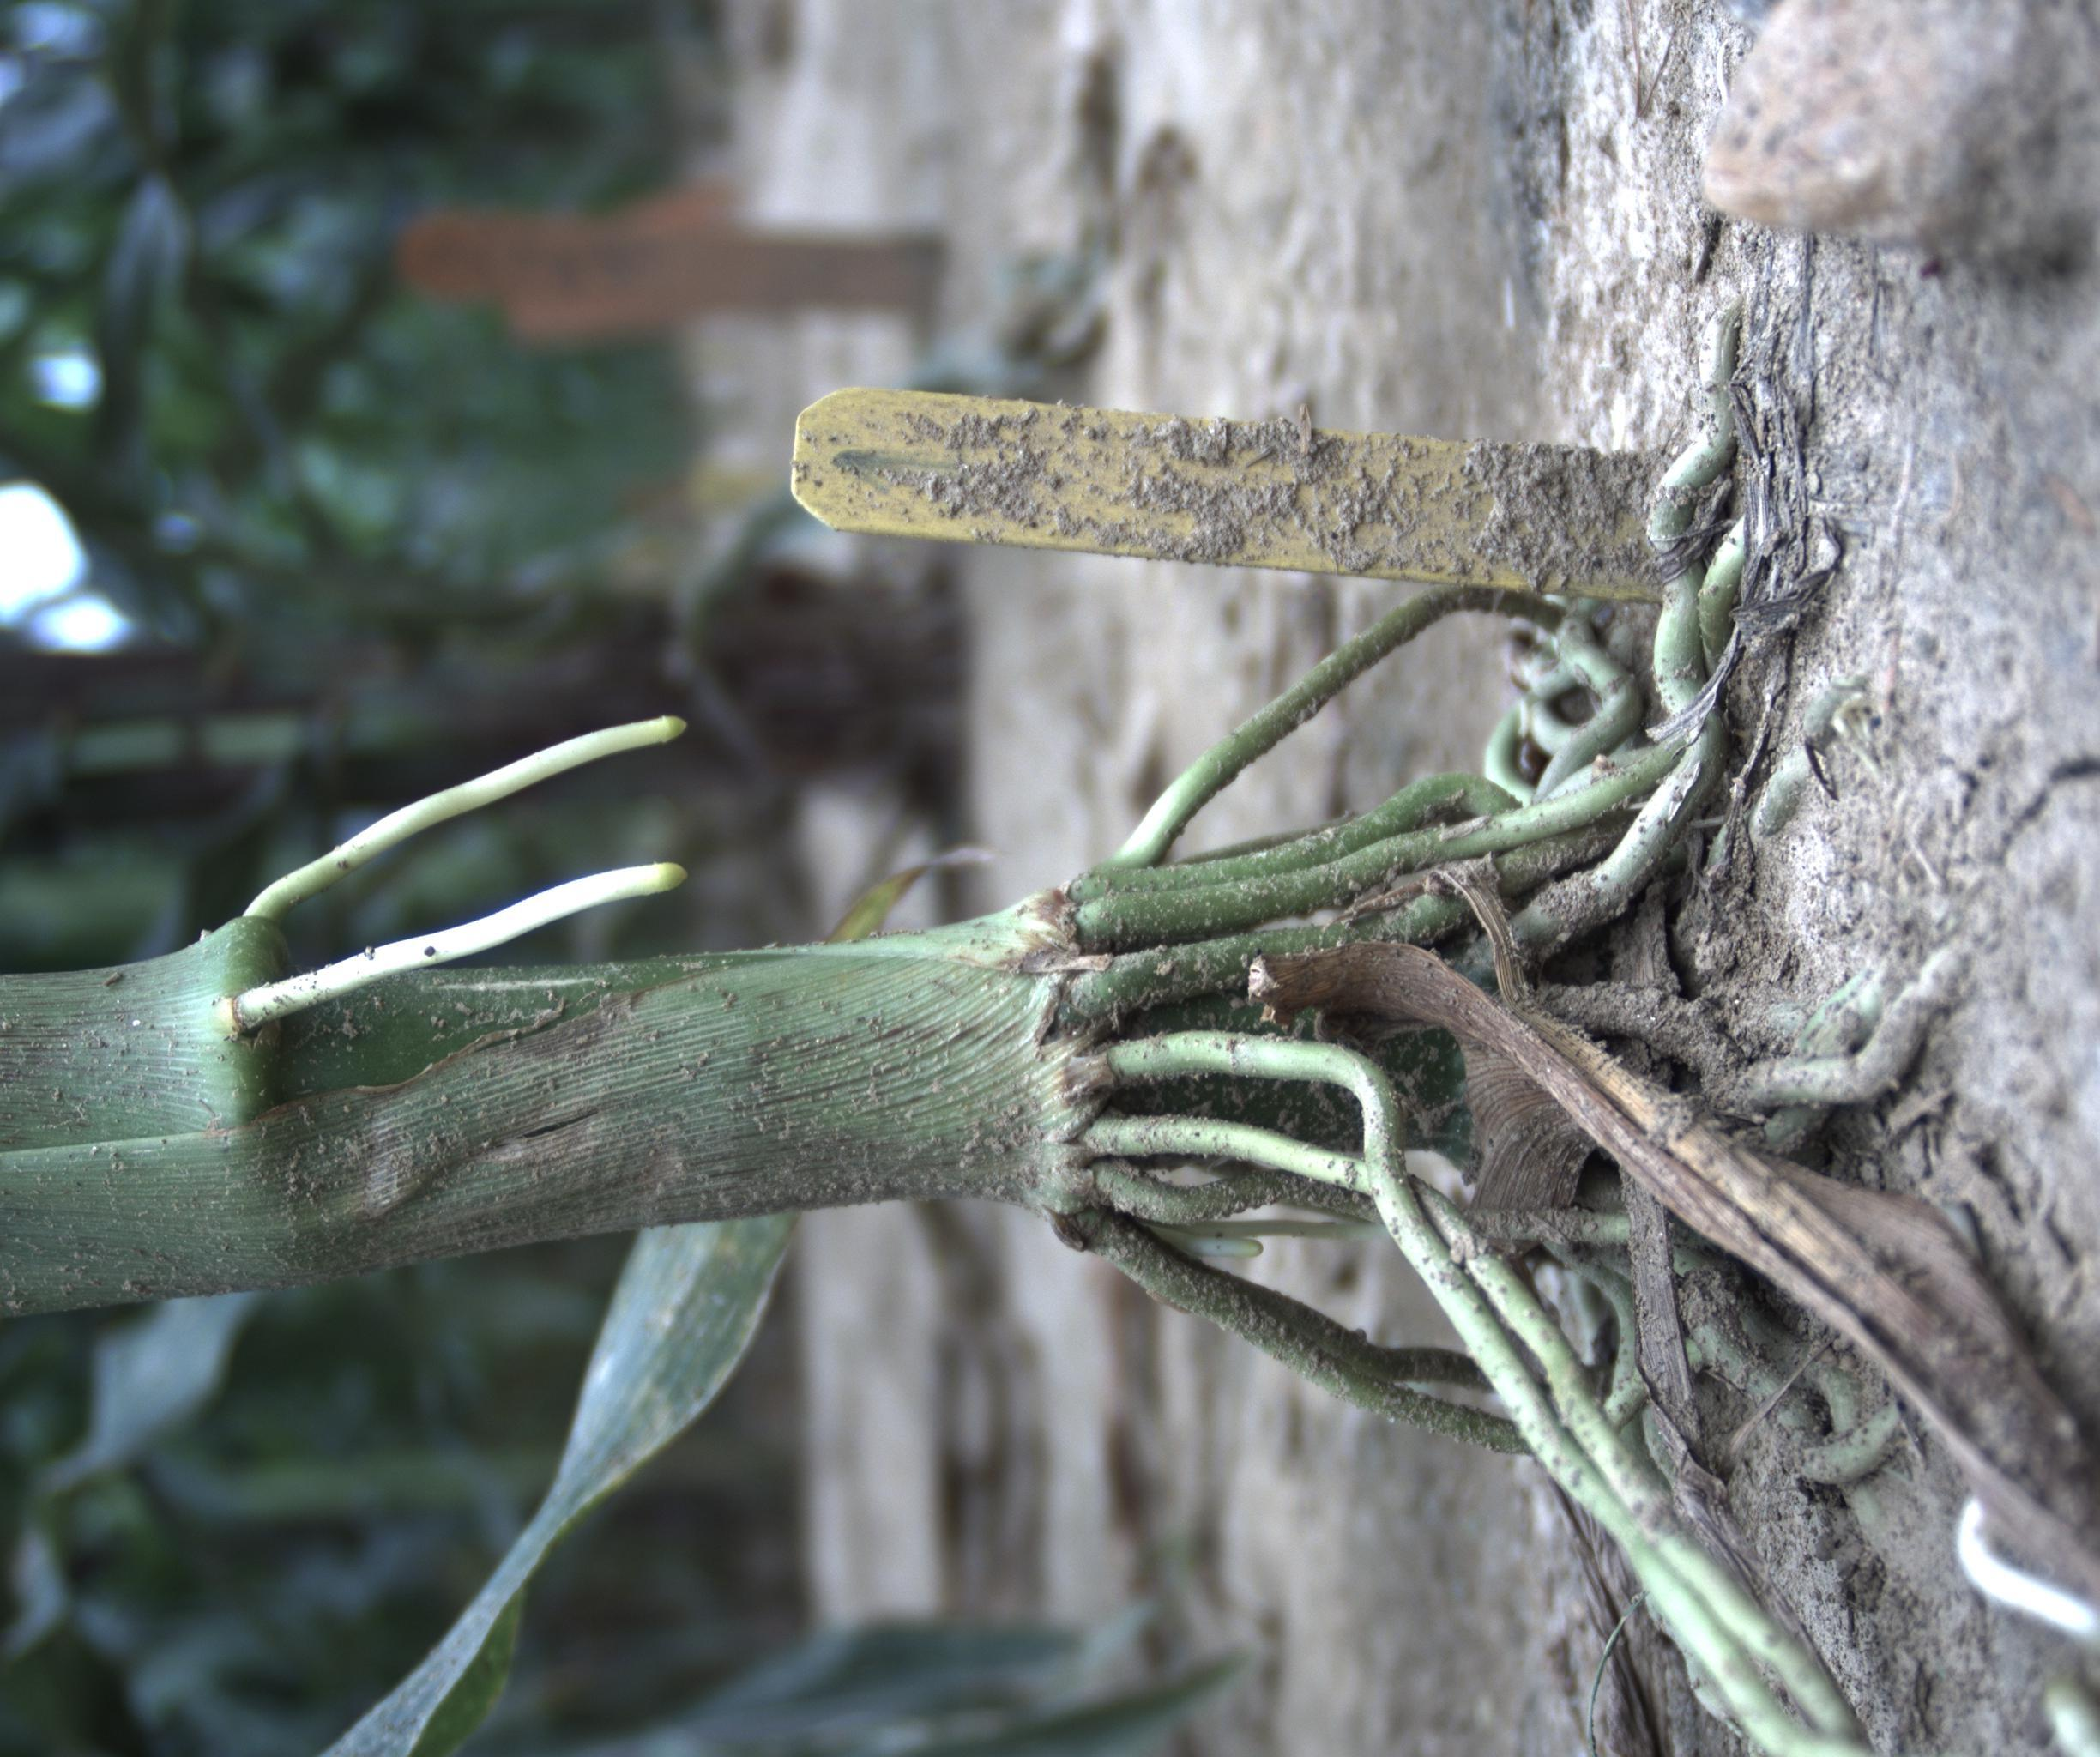
\includegraphics[width=\textwidth, angle=-90]{figures/w22.jpg}
    \end{minipage}
    \hfill
    \begin{minipage}{0.41\textwidth}
        \centering
        \includegraphics[width=\textwidth, angle=-90]{figures/TSH4.jpg}
    \end{minipage}
    \caption{TSH4 Mutants (right) show higher brace root counts than wild type (left) as well as more aerial brace roots and a secondary emergence pattern}
    \end{mdframed}
\end{figure}

With this in mind, it is hypothesized that TSH4 has a similar function in maize brace roots to its function in leaves and tassel bracts. That TSH4 acts as a stop signal and boundary for the organ development until the proper time for emergence. 

\section{Methods}
To test our hypothesis, we are seeking to follow some of the logic of Xiao et al.\cite{Xiao2022} We are using the CHipseq dataset from this paper and pairing it with out own whole node RNAseq analysis to see if the TSH4 targets are found in brace roots at each different stage of development. 

\subsection{CHiPseq}
The methods section of Xiao et al.\cite{Xiao2022} gives us this description of the CHiPseq experiment:
"Maize B73 plants were grown in the experimental field of the Plant Gene Expression Center, University of California Berkeley. Young ear primordia smaller than 5 mm were carefully dissected. About 1 g of tissue per biological replicate was fixed in 1 \% formaldehyde solution for 10 min under vacuum and quenched by adding glycine to a final concentration of 0.1 M. Nuclei extraction and ChIP using the TSH4 antibody were performed as described previously. \cite{Dong2019} Normal goat anti-rabbit IgG was used as a negative control. To validate the putative TSH4-binding targets, three biological replicates of immunoprecipitated DNA in ChIP were applied for each qPCR using respective primer pairs listed in table S13 (additional materials "xiao\_supplemental.xlsx") with Fast Evagreen qPCR mix. Relative enrichment was calculated using the $\delta$Ct (threshold cycle) method, and significant difference was evaluated through t test between anti-TSH4 ChIPed samples and IgG control." 
\subsection{Nodal RNAseq} 
For our nodal RNAseq dataset, samples from 3 nodes in each of 3 plant replicates were sequenced. Each of these 3 nodes representing a stage of brace root development. 


%begin Amaryllis-Methods
Samples were sent to Amaryllis Nucleics for processing and sequencing. RNA-seq libraries were prepared by using the Full Transcript mode YourSeq Dual (FT \& 3'-DGE) RNAseq Library Kit (Amaryllis Nucleics). A Bioanalyzer 2100 (Agilent, High Sensitivity DNA Kit) was used for library quality control, to determine average library size, and together with concentration data from a Qubit 2.0 Fluorometer (Life Technologies, dsDNA High Sensitivity Assay Kit) to determine individual library molarity and pooled library molarity. A PippinHT (Sage Science) was used for size selection to get pooled libraries 250-500 bp in length. These size-selected, pooled libraries were sequenced on a NextSeq 500 (Illumina, High Output v2 75 cycle kit) to yield single-read 80 bp reads. FASTQ sequence files were preprocessed in two steps. A Python library (clipper.py, https://github.com/mfcovington/clipper) was used to trim off the first 8 nucleotides of each read to remove potential mismatches to the reference sequence caused by annealing of a random hexamer required for library synthesis. Trimmomatic v0.36 \cite{Bolger2014} was used to remove adapter sequences and trim or filter reads based on quality. The parameters used for Trimmomatic were ILLUMINACLIP:TruSeq3-PE-2.fa:2:30:10 LEADING:3 TRAILING:3 SLIDINGWINDOW:4:15 MINLEN:50.

Preprocessed reads were mapped to the Zea mays B73 v4 genomic reference sequence \cite{nihMaysGenome} using HISAT2 \cite{HISAT2}. Read counts for each gene in the gene annotation file \cite{nihMaysGenome} were calculated using htseq-count (with the -s yes parameter to enforce strand-specific alignment) from the HTSeq Python library \cite{Anders2014}.

The R package edgeR \cite{edgeR} was used to identify genes differentially expressed between the three nodes of interest. Transcripts were retained for analysis if they had more than one count per million in at least three samples. After normalization factors were calculated and dispersion estimated, genewise negative binomial generalized linear models with quasi-likelihood tests were used to identify node effects across matched samples. Differentially expressed genes were then filtered using a false discovery rate (FDR) cutoff of 0.05. FDRs were calculated by adjusting P-values for multiple comparisons using the Benjamini–Hochberg procedure.
%end Amaryllis-Methods

The node highest on the plant, referred to as node 3, represents the Induction stage. This is the stage in which there are no observable brace root primordia. The second node from the ground, node 2, represents the initiation stage, where brace roots are just beginning to form emergence sights visible on the node. The lowest node to the ground, node 1, represents the Emergence stage, in which the brace roots have formed and are emerging from the plant and growing towards the soil.  
\begin{figure}[H]
    \centering
    \begin{mdframed}[backgroundcolor=green!20]
    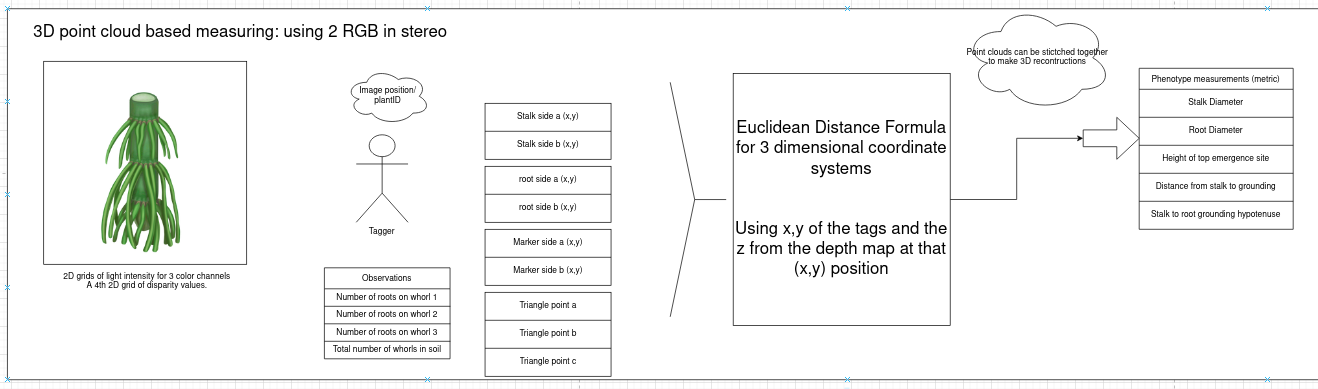
\includegraphics[width=1\linewidth]{figures/image.png}
    \caption{Stages of brace root development. Stage 1: Induction (signified as "node 3" in our analysis) shows no development. Stage 2: Initiation (signified as "node 2" in our analysis) shows when the brace root primordia start to form in the node. Stage 3: Emergence (signified as "node 1" in our analysis) shows when the brace root primordia emerges from the node. }
    \end{mdframed}
\end{figure}
\subsection{Enrichment analysis of differentially expressed TSH4 targets in brace root nodes}
The TSH4 Chipseq genes were converted from B73v3 to B73v4 using MaizeGDB gene mapping tool. \cite{Woodhouse2021} The converted list was used to filter each of the 3 DEG lists from RNAseq. Through a Venn diagram, the overlap gene set was divided into 7 subsets which were enriched through Agrigov2 \cite{Tian2017}. Gene ontology terms that were significantly enriched were noted and expression patterns for those genes were plotted in a heatmap of expression z-score.

\section{Results}
%Overlap Venn diagram
\subsection{TSH4 targets are differentially expressed between brace root nodes}
Of the 1392 TSH4 targets, 862 were present in our RNAseq dataset. 315 of those genes were differentially expressed between nodes with a log fold change of 1 or higher and an FDR below 0.05. \ref{fig:Venn1} shows a venn diagram of these gene sets. The overlap regions of this diagram signify subsets of interest because they are genes up or down regulated in a specific node. The regions on the perimeter of the diagram signify genes that transition between nodes or, in the case of the n3-n1 perimeter region, an end to end comparison. 
\begin{figure}[H]
    \centering
    \begin{mdframed}[backgroundcolor=green!20]
    \centering
    \includegraphics[width=.5\linewidth]{figures/venn_diagram.png}
    \caption{Venn diagram of TSH4 targets in nodal DEG list. Each of the 3 circles is a list of differentially expressed TSH4 targets. Naming for the sets includes the two nodes that were compared. Example: n3-n1 are DEG between node 3 (inductance) and node 1 (emergence)}
    \label{fig:Venn1}
    \end{mdframed}
\end{figure}

\subsection{Gene ontology reveals biological processes in brace root development}
%labeling the regions through GO report
For each of the 7 subsets of our overlapping gene set, only the epicenter of the venn diagram contained no significant GO annotations. The biological processes present in each subset confirms our logic previously described. The induction subset showed that there were large changes in anatomical structure morphogenisis (31 genes, GO:0009653) and post-embryonic development (28 genes, GO:0009791) to come in the next stages. The initiation subset showed no significant biological processes but showed changes in regulatory region nucleic acid binding (5 genes, GO:0001067) and transporter activity (10 genes, GO:0005212).  
The emergence subset contained clusters of GO terms indicating developmental growth involved in morphogenesis (9 genes, GO:0060560). Other ontology clusters include genes involved in the reproductive process (21 genes, GO:0022414), regulation of hormone levels (9 genes, GO:0010817) and steroid biosynthesis (5 genes, GO:0006694). The perimeter regions align well with transitions between stages of brace root development with changes from induction to initiation showing the beginnings of lateral organ development and changes from initiation to emergence being marked with regulation of gene expression. The end to end comparison marked significant changes in metabolism and cell signaling.   
\subsection{Expression patterns of TSH4 \& signalling pathways suggest regulation}
Expression of TSH4 is very high in inductance becomes down regulated in initiation and is not significantly expressed in emergence. This mirrors the pattern found in tassel bracts and suggests that TSH4 is suppressing brace root development. In tassel bracts, two signalling pathways, gibberellin and auxin, are found to be attenuated by TSH4 while abscisic acid is promoted.\cite{Xiao2022} In brace roots we do not see the same hormone signals but we do see signals involved in root growth: Ethylene, auxin, and brassinosteroids. In \ref{fig:meta-express} we can see that ethylene and brassinosteroids have an inverse expression pattern to TSH4, this suggests a suppression interaction.  
\begin{figure}[H]
    \centering
    \begin{mdframed}[backgroundcolor=green!20]
    \centering
    \includegraphics[width=.95\linewidth]{figures/Hormonal_expression_heatmap.png}
    \caption{Expression heatmap (by z-score) across nodes shows that TSH4 expression is high in node 3 and metabolic signals such as BRS1 (Brassinosteriod synthesis 1) and EREB118 (ethylene responsive element binding protein 118) show an inverse expression pattern to TSH4. In contrast to tassle bracts, Auxin response factor transcription factors (ARFTF) are co-expressed with TSH4}
    \label{fig:meta-express}
    \end{mdframed}
\end{figure}
\subsection{The presence of other transcription factors suggest a regulatory network}
In \ref{fig:meta-express} we saw a auxin response factor transcription factors were highly expressed with TSH4 in the induction stage of brace root development. But there are also other transcription factors that have interesting expression patterns. Notably, myoblastosis transcription factor 99 (MYB99) and heatshock transcription factor 18 (HSFTF18) have the inverse expression pattern of TSH4. MYB99 is a key transcription factor in regulating secondary metabolic processes. \cite{Cao2020} HSFTF18 has also been found to be expressed in brace roots. \cite{Li2019} 
\begin{figure}[H]
    \centering
    \begin{mdframed}[backgroundcolor=green!20]
    \centering
    \includegraphics[width=.95\linewidth]{figures/TF_expression_heatmap.png}
    \caption{Expression heatmap (by z-score) across nodes shows that TSH4 expression is high in node 3 and the presence of other TFs show that there may be more complicated regulation networks at play.}
    \label{fig:meta-express}
    \end{mdframed}
\end{figure}


\section{Discussion}
More work is required in order to find the exact mechanisms of tassel sheath 4's regulation of brace root development. But this data does suggest that a similar pattern to the one in tassel bracts. We see suppression of many genes involved in organ development and massive metabolic and signalling changes throughout all three stages. It should be noted that a good way to improve this study is to get both sequencing data sets from the same part of the plant, ie. running the CHiPseq experiment using brace root tissue. This could filter out TSH4 targets that are specific to flowering. Another possible way to continue from this point would be to try to find possible links in the regulatory chain by trying to predict interactions amongst the un-characterized gene products in this data set. With this in mind, the results of this project show promising evidence for a regulatory network around brace root development and justifies further investigation.   




\printbibliography

     % This file (appA.tex) contains the text
                   % for Appendix A. 
 
\include{appB}     % This file (appB.tex) contains the text
                   % for Appendix B.   
       
\end{document}